%%%%%%%%%%%%%%%%%%%%%%%%%%%%%%%%%%%%%%%%%%%%%%%%%%%%%%%%%%%%%%%%%%%%
%% I, the copyright holder of this work, release this work into the
%% public domain. This applies worldwide. In some countries this may
%% not be legally possible; if so: I grant anyone the right to use
%% this work for any purpose, without any conditions, unless such
%% conditions are required by law.
%%%%%%%%%%%%%%%%%%%%%%%%%%%%%%%%%%%%%%%%%%%%%%%%%%%%%%%%%%%%%%%%%%%%

\documentclass[
  digital,     %% The `digital` option enables the default options for the
               %% digital version of a document. Replace with `printed`
               %% to enable the default options for the printed version
               %% of a document.
%%  color,       %% Uncomment these lines (by removing the %% at the
%%               %% beginning) to use color in the printed version of your
%%               %% document
  oneside,     %% The `oneside` option enables one-sided typesetting,
               %% which is preferred if you are only going to submit a
               %% digital version of your thesis. Replace with `twoside`
               %% for double-sided typesetting if you are planning to
               %% also print your thesis. For double-sided typesetting,
               %% use at least 120 g/m² paper to prevent show-through.
  nosansbold,  %% The `nosansbold` option prevents the use of the
               %% sans-serif type face for bold text. Replace with
               %% `sansbold` to use sans-serif type face for bold text.
  nocolorbold, %% The `nocolorbold` option disables the usage of the
               %% blue color for bold text, instead using black. Replace
               %% with `colorbold` to use blue for bold text.
  lof,         %% The `lof` option prints the List of Figures. Replace
               %% with `nolof` to hide the List of Figures.
  lot,         %% The `lot` option prints the List of Tables. Replace
               %% with `nolot` to hide the List of Tables.
]{fithesis4}
%% The following section sets up the locales used in the thesis.
\usepackage[resetfonts]{cmap} %% We need to load the T2A font encoding
\usepackage[T1,T2A]{fontenc}  %% to use the Cyrillic fonts with Russian texts.
\usepackage[
  main=english, %% By using `czech` or `slovak` as the main locale
                %% instead of `english`, you can typeset the thesis
                %% in either Czech or Slovak, respectively.
  english, german, czech, slovak %% The additional keys allow
]{babel}        %% foreign texts to be typeset as follows:
%%
%%   \begin{otherlanguage}{german}  ... \end{otherlanguage}
%%   \begin{otherlanguage}{czech}   ... \end{otherlanguage}
%%   \begin{otherlanguage}{slovak}  ... \end{otherlanguage}
%%
%%
%% The following section sets up the metadata of the thesis.
\thesissetup{
    date        = \the\year/\the\month/\the\day,
    university  = mu,
    faculty     = fi,
    type        = bc,
    department  ={Department of Computer Systems and Communications},
    author      = Jindřich Halabala,
    gender      = m,
    advisor     = {RNDr. Ondřej Krajíček},
    title       = {Experimenting with web-page structural analysis using Deep Reinforcement Learning},
    TeXtitle    = {Experimenting with web-page structural analysis using Deep Reinforcement Learning},
    keywords    = {TODO, keyword2, ...},
    TeXkeywords = {TODO, keyword2, \ldots},
    abstract    = {%
      This is the abstract of my thesis, which can

      span multiple paragraphs.
    },
    thanks      = {%
      These are the acknowledgements for my thesis, which can

      span multiple paragraphs.
    },
    bib         = example.bib,
    %% Remove the following line to use the JVS 2018 faculty logo.
    facultyLogo = fithesis-fi,
}
\usepackage{makeidx}      %% The `makeidx` package contains
\makeindex                %% helper commands for index typesetting.
%% These additional packages are used within the document:
\usepackage{paralist} %% Compact list environments
\usepackage{amsmath}  %% Mathematics
\usepackage{amsthm}
\usepackage{amsfonts}
\usepackage{url}      %% Hyperlinks
\usepackage{markdown} %% Lightweight markup
\usepackage{listings} %% Source code highlighting
\usepackage{svg}      %% SVG figures
\lstset{
  basicstyle      = \ttfamily,
  identifierstyle = \color{black},
  keywordstyle    = \color{blue},
  keywordstyle    = {[2]\color{cyan}},
  keywordstyle    = {[3]\color{olive}},
  stringstyle     = \color{teal},
  commentstyle    = \itshape\color{magenta},
  breaklines      = true,
}
\usepackage{floatrow} %% Putting captions above tables
\floatsetup[table]{capposition=top}
\usepackage[babel]{csquotes} %% Context-sensitive quotation marks
\begin{document}
%% The \chapter* command can be used to produce unnumbered chapters:
\chapter*{Introduction}
%% Unlike \chapter, \chapter* does not update the headings and does not
%% enter the chapter to the table of contents. I we want correct
%% headings and a table of contents entry, we must add them manually:
\markright{\textsc{Introduction}}
\addcontentsline{toc}{chapter}{Introduction}

TODO

\chapter{User interface element detection}

Y Soft AIVA\footnote{\url{https://www.ysoft.com/aiva}} is a software solution for automated end-to-end testing of web applications. Unlike most competitors, AIVA does not interact with or read a web page's Document Object Model (DOM). Instead, it relies entirely on visual information. This approach closely resembles how a real user interacts with the application (black-box testing) and enhances robustness in specific scenarios, such as when XPaths change due to newly added components. However, it also presents many challenges since all the information must be extracted from an image instead of a markup language.

A crucial aspect of data extraction is identifying the location, size, and hierarchical relationships of all key interactable elements on a web page (e.g., buttons, icons, text fields). If this step is done well, it allows AIVA to reconstruct the DOM and localize correct elements during test execution.

This process can be approached using both detection and segmentation, as most objects on a webpage are rectangular. However, due to the hierarchical nature of the DOM, detection is a more intuitive choice, as a single pixel can belong to multiple overlapping elements. That said, the detected information can be converted into a segmentation map if needed. This correspondence is visible in \autoref{fig:example-result}.

\begin{figure}
    \centering
    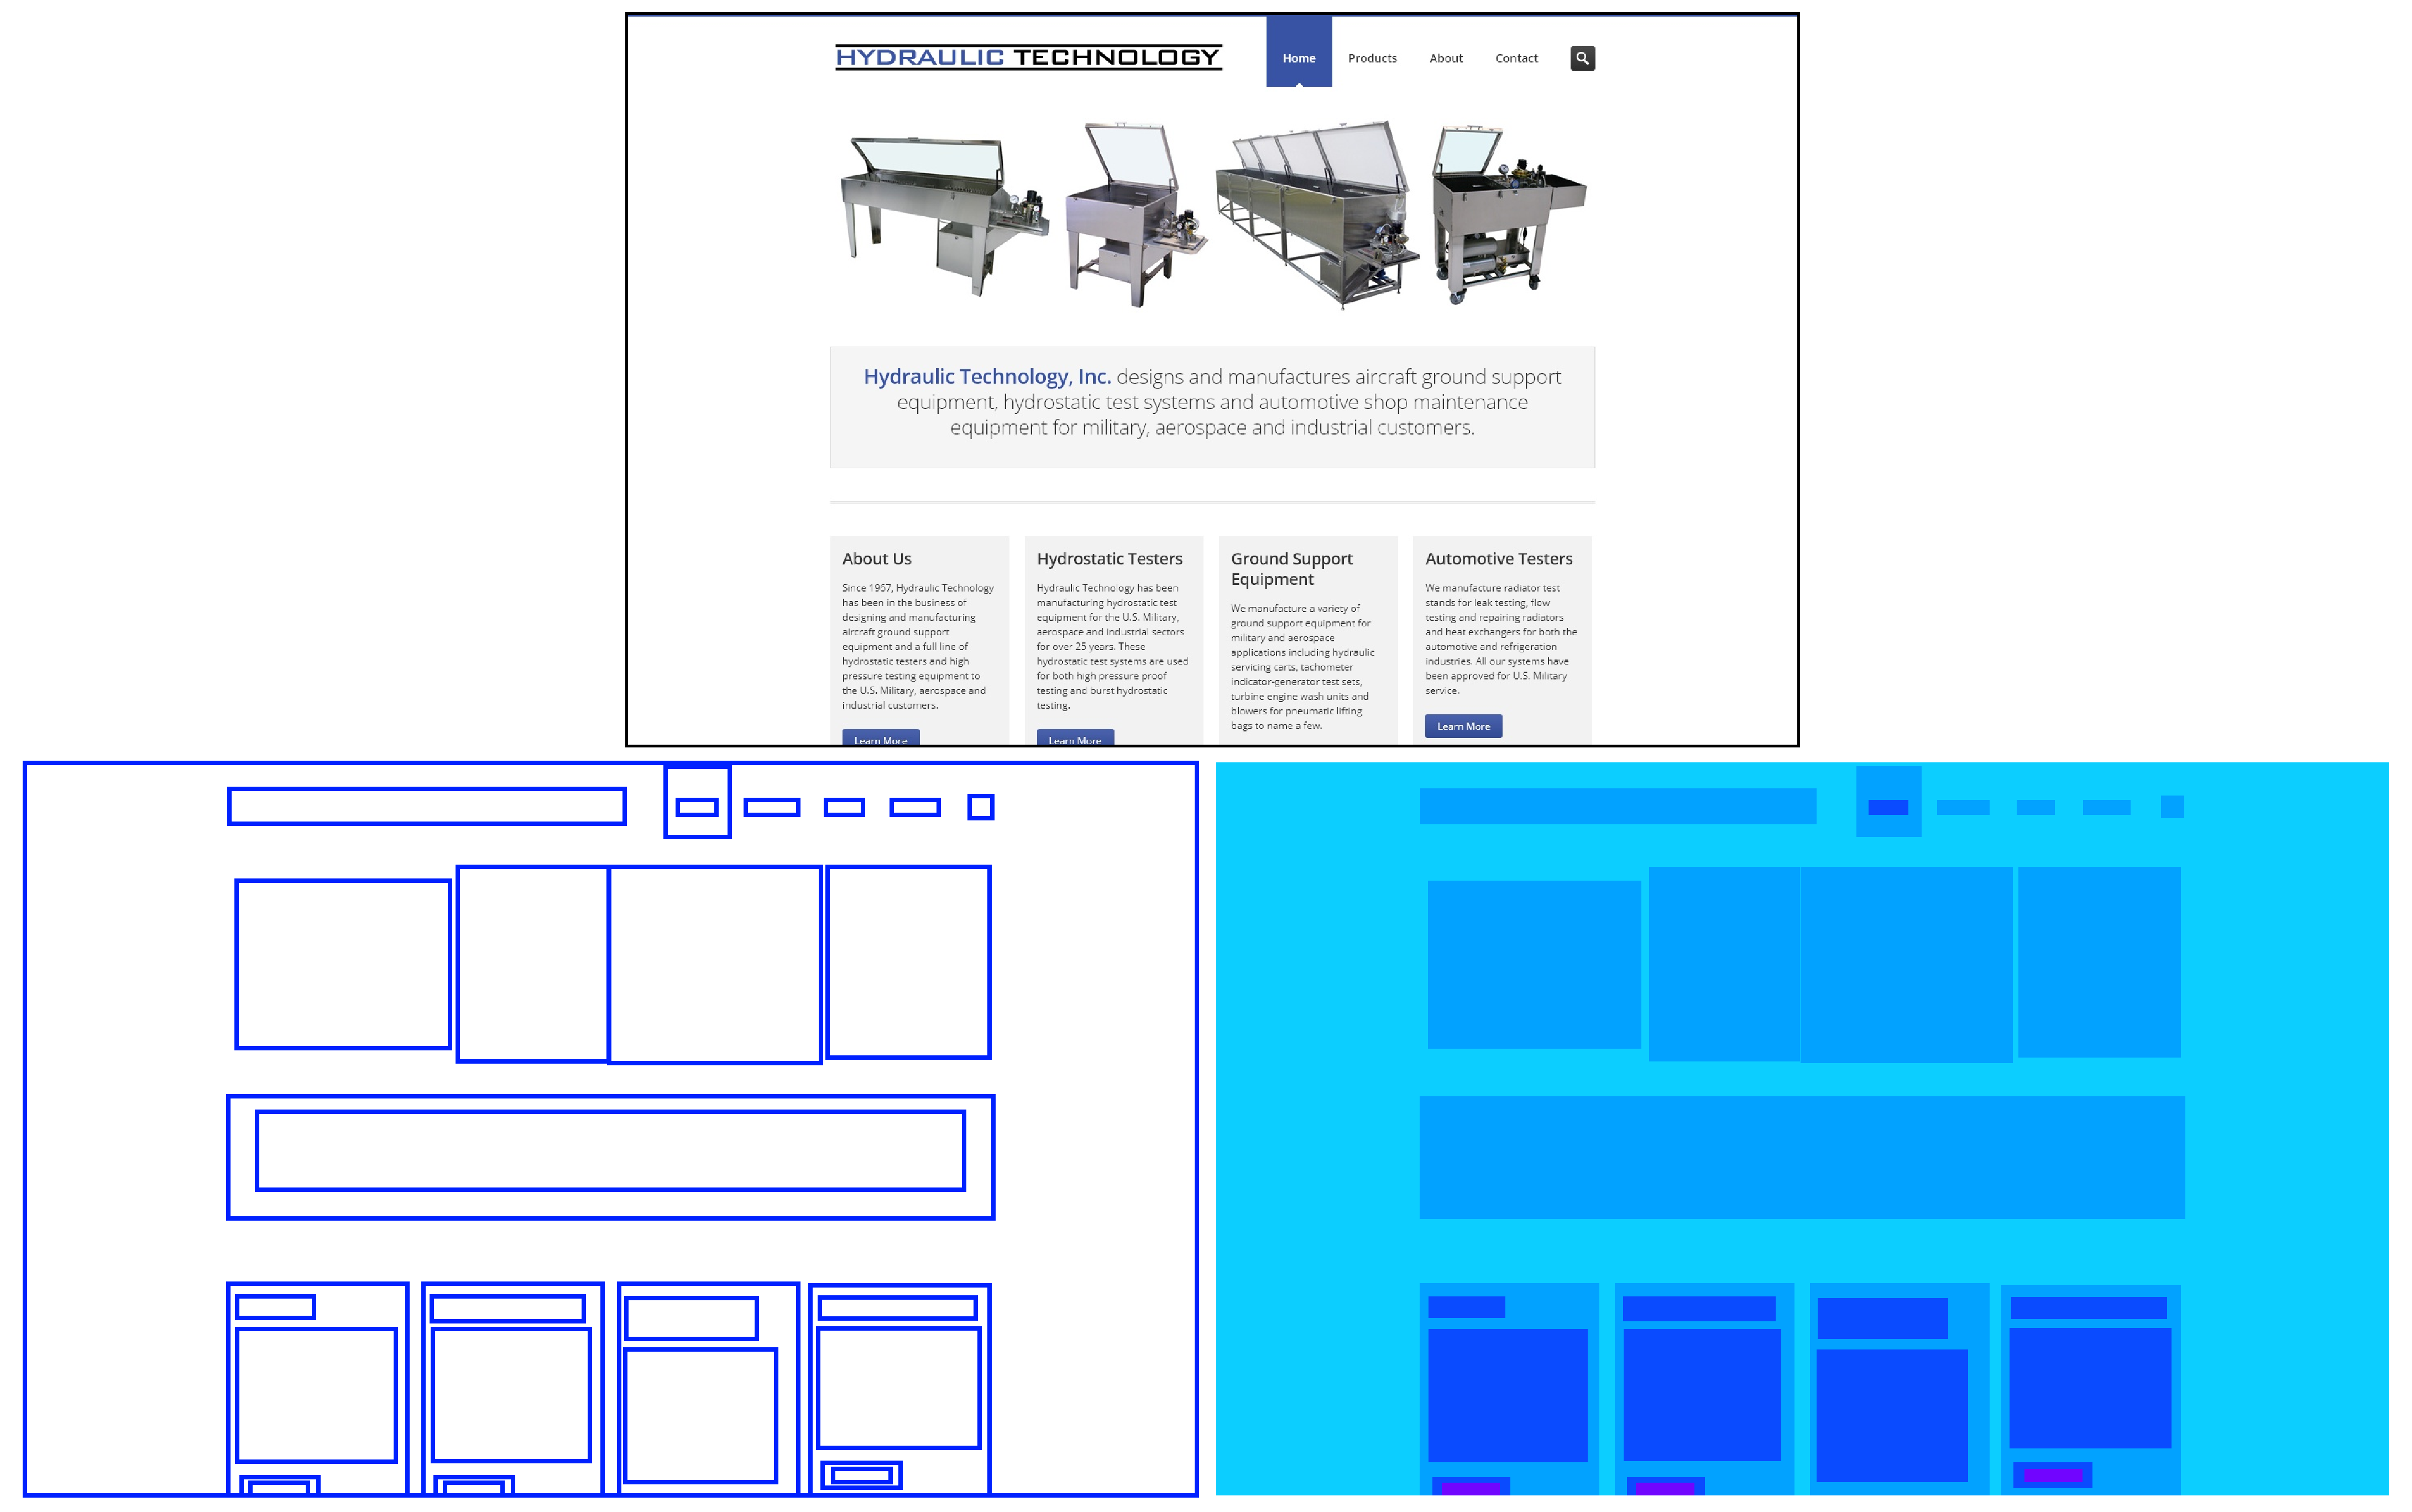
\includegraphics[width=1\linewidth]{diagrams/result_example.pdf}
    \caption{An example of an ideal result. The top image is the original screenshot, the bottom left shows bounding boxes of detection, and the bottom right shows the same as a segmentation map. The original image comes from \cite{aydos2020}.}
    \label{fig:example-result}
\end{figure}

User interface (UI) object detection such as this is done either using traditional computer vision (CV) or by deep learning-based object detection models such as R-CNNs or YOLO or by combining both (for example, using a DL model for text and image detection and CV for the rest) \cite{ODforGUI_CV_DL_or_both}. This chapter looks at both approaches, some existing solutions based upon them, and the challenges they present. Finally, a third approach that could solve these problems is proposed based on deep reinforcement learning.

\section{Traditional computer vision-based solutions}

Traditional computer vision is used in this thesis to describe algorithms for digital image processing that do not utilize machine learning, instead operating on a pixel-by-pixel basis. Tradition CV is not ideal for object detection in photographs due to noise and unclear edges but is well-suited for processing user interfaces. Screenshots usually do not contain any noise (at most, some compression artifacts might be present), and edges are clearly defined.

The most common technique is using an edge detection method (e.g., Canny or Sobel edge detection) followed by some extra processing to make the edges cleaner (e.g., morphological operations, filtering of small edges), and finally, detecting contours in the binary image. This process is then commonly combined with results from an optical character recognition (OCR) model and further processed to merge similar elements and filter out small elements that are likely just noise. We can find this exact process in algorithms such as REMAUI \cite{remaui} (a program for reverse engineering of mobile application UIs), UISeg \cite{uiseg} (user interface segmentation algorithm), and also in the current implementation of AIVA's element detection procedure.

Template matching is another approach for localization, but it lacks flexibility. It works well for highly standardized elements (e.g., checkboxes or buttons in desktop applications with a fixed UI). However, it is ineffective for mobile or web applications where UI components vary widely in design \cite{ODforGUI_CV_DL_or_both}.

Even today, with the rapid progress in deep learning (DL), traditional CV still has many benefits. It can be much more efficient and straightforward to understand, making it much easier to modify and debug. We can observe the results of each step of an algorithm, see what went wrong, and adjust parameters and thresholds accordingly. These sorts of modifications are not possible (or at least not simple to do) with DL. Another significant benefit is not having to create a large dataset for training, which often requires a lot of manual labor, and even then, it could be of low quality, making it impossible to train a good model. This also makes CV-based solutions a lot more flexible -- trends in user interface design tend to change rather quickly, making older datasets obsolete  \cite{DLvsTCV}.

\section{Deep learning-based solutions}
In the last ten years, state-of-the-art object detection algorithms have been almost solely based on deep neural networks with convolutional layers. Region-based Convolutional Neural Networks (R-CNNs) and You Only Look Once (YOLO) are the two most prominent model families. Generally, R-CNNs offer higher accuracy, while YOLO provides better speed, though performance varies by model and use case \cite{ObjectDetectionHistorySurvey}.

An example of a deep learning-based UI element detection algorithm is OmniParser -- a fine-tuned YOLOv8 model for parsing and labeling UIs. It was created to improve the performance of large multi-modal agents like GPT-4V \cite{OmniParser}. \cite{GUI_YOLO_comparison} tried training different YOLO architectures for UI element detection with good results. When AIVA was primarily used to test physical devices with touch screens, it used a model based on the Single Shot Detection architecture for element detection \cite{Horak2020thesis}.

A key advantage of DL-based solutions is that they do not require manual tuning for a specific domain. They can also detect complex patterns without explicit programming. With a large enough high-quality dataset and proper model architecture, almost anything can be learned automatically from the data. However, as stated in the previous section, this is also one of the main drawbacks. It is also way more demanding on hardware, especially for training \cite{DLvsTCV}.

\section{Object detection with reinforcement learning}

The previous two sections highlight two significant challenges. Traditional CV is insufficient for more complex images, and DL requires a large, high-quality dataset. Could we somehow combine these two methods to eliminate or at least mitigate these drawbacks? It should be possible to create a function that judges the quality of a bounding box prediction based on traditional CV and then use it to train a DL model. This approach eliminates the need for a dataset with ground truth bounding boxes, requiring only images of web applications, which are significantly simpler to obtain.

Supervised learning models are not applicable if we only have a numerical score for predictions rather than ground truth labels. Instead, we can use a reinforcement learning model that learns from evaluative feedback (more details on RL in \autoref{chap:dlr}).

My research shows that there have been no attempts at multi-object detection using reinforcement learning. However, there have been papers on using it to detect a single object in photographs \cite{dlr_object_detection, iterative_od_with_rl, hierarchical_od_with_drl} and for region proposal in multi-object detection \cite{drl_rpn}. They all use ground-truth labels for learning, but I believe this is because creating a CV-based reward function for photographs would be very difficult. However, for UIs, it should be feasible. 

\chapter{Deep reinforcement learning}
\label{chap:dlr}

To understand the terminology used and decisions made in the following chapters, it is important to first have a basic understanding of the theory behind reinforcement learning and machine learning in general. This chapter should provide enough information to understand the rest of this thesis. Please note that it is only a brief introduction to the topic; only the most important algorithms and definitions are provided. It is definitely not exhaustive.

Unless stated otherwise, the notation and information used in this chapter are from the book \textit{Grokking Deep Reinforcement Learning} by Miguel Morales \cite{GDRL}.

\section{Machine learning}
Machine learning (ML) is the study of algorithms that allow computers to learn from data without explicit programming. It is often split into three main categories: supervised learning, unsupervised learning, and reinforcement learning (note that other categories, such as semi-supervised or self-supervised learning, are also sometimes stated, but they are usually just modifications of the three main categories) \cite{IB031}.

In supervised learning (SL), the goal is to learn to make predictions when the correct answers are available during training. This is ideal for classification or regression, where we are able to get the correct labels (be it from human labeling, automated data collection, or some other method) \cite{IB031}.

In unsupervised learning (UL), no correct labels are known, so it is more about finding patterns in the provided data. This can be used to, for example, separate the data into groups (clustering) or to generate new data similar to the provided examples (autoencoders, generative adversarial networks) [ZDROJ???? Asi IB031 pro definici a PV021 pro příklady].

Just like SL, reinforcement learning predicts labels for some input data, but unlike in SL, the correct answers are not known. Instead, the learning is done using a reward function, which is able to score how good or bad the prediction was. The goal is to then learn to make decisions that maximize this reward through trail and error. This makes RL ideal for decision-making, especially in environments where we do not have access to the optimal strategy.

\section{Reinforcement learning}
Reinforcement learning problems are composed of two entities that interact -- the agent and the environment. The agent is the algorithm we are trying to teach to make decisions. The environment is everything else -- if the goal is to drive a car, then the environment is all the other cars, how they move, all the roads, pedestrians, but also the car the agent is controlling. The agent interacts with the environment through its decisions and tries to do this in such a way that maximizes the reward.

We define the RL cycle. In the beginning, the environment is in some initial state. The agent observes the state and, based on this observation, decides to perform an action. The environment then reacts to this action, changing its inner state. The agent then observes the new state and also receives a reward based on the action. The agent can then learn and change its behavior based on the reward. It then again chooses an action, and the cycle repeats as can be seen in figure \ref{fig:rl-cycle}.

\begin{figure}
    \centering
    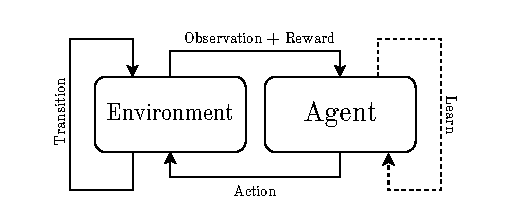
\includegraphics[width=1\linewidth]{diagrams/rl_cycle.pdf}
    \caption{Reinforcement learning cycle}
    \label{fig:rl-cycle}
\end{figure}

One iteration of this cycle is called a time step and creates an experience -- a tuple of the original state $s$, the action taken $a$, the reward given $r$, and the new state $s'$. Depending on the task this cycle can repeat forever or end, once the environment reaches some terminal state. For example, in a game of chess, the end is defined as winning, losing, or a draw. We call such tasks episodic, and all the experiences collected from the initial to the terminal states form an episode. If there is no well-defined end, we call a task continuous. For example when we teach a robot to walk there is no goal, we just want it to walk the furthest or the fastest.

Reinforcement learning is challenging due to the feedback being sequential, evaluative, and sampled.

The sequentiality comes from most of the tasks being multiple steps long, and thus, the consequences of an action might not be apparent immediately. When an episode ends with a very negative result it can be hard to figure out which of the preceding actions is the cause as it often is not the last action taken.

Feedback being evaluative means that the reward given is just a number. Without additional context it is impossible to know if the received reward was the best possible and we should thus repeat the decision in similar states or whether it was terrible and should be avoided in future. This leads to the need for exploration discussed in \autoref{sec:eplor-exploit}.

Lastly, sampled feedback. We only know the reward we received for the states and actions we actually tried, and in most cases, there are so many states that it is impossible to try every combination of state and action. Also, often the observation does not contain the entire state; only some part of it. Of course, this is a problem even in supervised learning, as the dataset will never contain all the data that we might encounter in the future.

\section{Markov decision process}
In order to formally define RL and its goal, we first have to formally define the environment. There are multiple ways in which we can define an environment, but the most common representation is a Markov decision process (MDP). Formally, MDP is defined as a tuple $(S, A, p, r)$.

$S$ is the set of all possible states of the environment -- the state space. It can be both discrete (in chess, there is a finite amount of pieces that can be located in a finite amount of positions) or continuous (the speed of a car or its position can be any real number).  At each time step t, the MDP is in a state $s_t\in S$.

$A$ is a set of all possible actions that can be done by the agent -- the action space. Again, it can be both discrete or continuous (or a combination of both).

$p$ is the probabilistic transition function $p\colon S \times A \to \mathcal{D}(S)$ that, for a given state $s$ from $S$ and a given action $a$ from $A$, returns a probability distribution over the states $s'\in S$ which tells us the probability of the MDP transitioning from $s$ to $s'$ given that action $a$ was selected. Formally it can be defined as:
\[
p(s'|s,a)=P(S_t=s'|S_{t-1}=s,A_{t-1}=a)
\]
Of course, since we are dealing with probabilities, we want the sum of all the probabilities for a given state $s$ and action $a$ to be equal to one:
\[
\sum_{s'\in S} p(s'|s,a)=1, \forall s \in S, \forall a \in A
\]
In practice, some action a might not be possible in a state $s$, but we can solve this problem by setting the probability of $p(s|s, a) = 1$ and $p(s' | s, a) = 0, \forall s'\in S \setminus s$ -- the MDP will \enquote{transition} back into the original state with a probability of one if such action is chosen.

Lastly, $r$ is the reward function. Depending on the use case, it can be defined either as $r\colon S \times A \to \mathbb{R}$ -- the expected reward given for choosing action $a$ in state $s$:
\[
r(s,a)= \mathbb{E} [R_t|S_{t-1}=s, A_{t-1}=a]
\]
\cite[p. 17, p. 54]{PA230, GDRL} or as $r\colon S\times A \times S \to \mathbb{R}$ -- the expected reward given for choosing action $a$ in state $s$ given we transition into state $s'$:
\[
r(s, a, s')= \mathbb{E} [R_t|S_{t-1}=s, A_{t-1}=a, S_t=s']
\]
\cite[p. 54]{GDRL}
Which one we choose depends on the task we are solving. The main distinction is whether we only care about transitioning from one state to the other or if we also care about how that transition was achieved. For example, when driving a car, we might want to reward differently braking using the engine and braking using the brakes -- they both achieve the same thing (the resulting state is the same), but they were achieved using a different method (different action).

Another thing that is often defined is the set of initial states $S^i \subseteq S$. When a MDP is initialized, the initial state is chosen from this subset using some probability distribution $\mathcal{I}$ over these states. Of course, we can omit defining the set $S^i$ and just make the probability of all the other states zero. \cite[p. 50]{GDRL}

Similarly, a set of all terminal states can be defined. The MDP ends when it gets into one of the terminal states. But once again, we can omit this by defining the transition function in such a way that every transition from a terminal state has a probability of 1 of transitioning back into the state itself and by ensuring that such transition always has a reward of 0.
Simple MDPs can be visualized as diagrams, as can be seen in figure \ref{fig:mdp}.

\begin{figure}
    \centering
    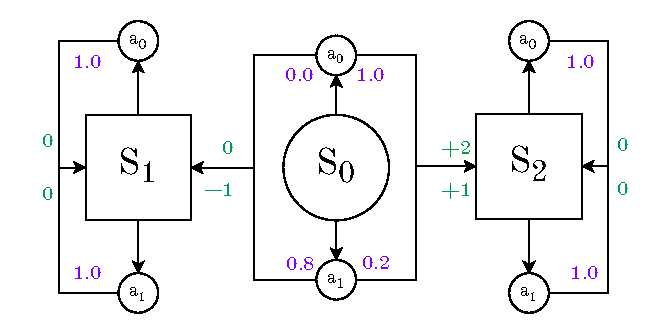
\includegraphics[width=1\linewidth]{diagrams/mdp.pdf}
    \caption{Markov decision process. Terminal states are depicted by squares. Transition probabilities are purple; rewards are green.}
    \label{fig:mdp}
\end{figure}

\subsection{Markov property}
Notice that the probabilistic transition function $p$ only takes the current state and action as input. Importantly, it does not take history into consideration. The probability of transitioning from state $s$ to state $s'$ using action $a$ is always the same no matter how we got into the state $s$. This memorylessness of MDPs is known as the Markov property \cite[p. 49]{GDRL}, and it is important to remember when implementing an environment since many RL algorithms rely on the environment to fulfill the Markov property. It can be formally defined as
\[
P(S_{t+1}|S_t,A_t)=P(S_{t+1}|S_t,A_t,S_{t-1},A_{t-1}, \dotsc)
\]
An example of an environment that breaks this property could be the game of Pong\footnote{\url{https://en.wikipedia.org/wiki/Pong}} where the state is only the current frame. From just one frame, it is not possible to know which way or at what speed the ball will move after the next input. We can, of course, easily fix this by including not only the position but also the speed and direction of the ball in the state (or using other techniques such as frame-stacking, where we include multiple frames in the observation). In real-world scenarios, fully capturing movement may require including higher-order dynamics like acceleration or jerk. However, in practice, modeling up to acceleration is typically sufficient for most RL tasks.

\subsection{MDP modifications}
It should be mentioned that there are many possible extensions for MDPs that could be necessary for representing actual environments, such as continuous time MDPs, which do not operate on discrete time, or multi-agent MDPs, which allow multiple agents to interact with the environment at the same time. \cite[p. 59]{GDRL}

One extension that I want to talk about more is partially observable MDP (POMDP). As mentioned earlier, in most cases, the agent does not see the entire state of the MDP it interacts with, but only some part of it -- an observation. To account for this, we add two more properties into the tuple defining the MDP -- $\mathcal{O}$ and $\epsilon$. $\mathcal{O}$ is the set of all possible observations -- observation space. $\epsilon$ is a function $S \to \mathcal{D}(\mathcal{O})$ -- for a given state $s$ it returns a probability distribution over the observation space. However, to make things simpler, we will consider only regular MDPs for the rest of this chapter.

\section{Policy}
Now that we have formally defined the environment using a MDP, we can also formally define the agent. We can imagine the agent as some entity that receives a state $s$ and, based on it, chooses an action $a$ that is then performed, and the agent receives a reward $r$ and a new state $s'$. As already mentioned, we call the tuple $(s, a, r, s')$ an experience. The entire chain of these experiences is called a trajectory $\tau$, and since the ending state of one experience and the initial state of the following experience is always the same, we can write it only once: $s_0,a_0,r_1,s_1,a_1,r_2,\dotsc \in (S\cdot A \cdot \mathbb{R})^{*}$. Note that a trajectory is infinitely long since even in a terminal state, we can still perform an action; it just won't give us any reward or transition the environment into a different state. History is then some prefix of trajectory ending in a state: $s_0,a_0,r_1,s_1,a_1,r_2,\dotsc, a_{t-1},r_t,s_t\in (S\cdot A \cdot \mathbb{R})^{*}\cdot S$. The agent has to make the decisions based on some rules. We call policy $\pi$ a function $\pi\colon (S\cdot A \cdot \mathbb{R})^{*}\cdot S \to \mathcal{D}(A)$, which returns a distribution over the action space based on the history up to that point \cite[p. 19]{PA230}.

If we assume that the Markov property is fulfilled, we can simplify policy to just $\pi\colon S \to \mathcal{D}(A)$ because in that case, we know that the environment is memoryless, and thus, it does not matter how we ended up in the state $s_t$. Thanks to this, our agent (and its underlying policy) can be memoryless as well. Note that this is only true if we receive the entire state, so this simplification can not be applied to POMDPs (two different states might produce the same observation, and the history might help us differentiate between them).

We can further simplify the policy by making it deterministic -- instead of returning a probability distribution $\mathcal{D}(A)$ it returns just a single action $a$. Such policy can be defined as just $\pi\colon S \to A$.

\section{The goal of RL}
\label{section:goal}
Now that we have fully formally defined the environment (MDP) and the agent (policy), we can define the goal of RL. The goal is to find such a policy $\pi^*$ that maximizes the expected discounted cumulative reward, also referred to as the discounted return. The cumulative reward of a trajectory $\tau$ is defined as the sum of all received rewards:
\[
r_1+r_2+r_3+\dotsb = \sum_{i=0}^{\infty} r_{i+1}
\]
To get the discounted return, we exponentially decay the rewards by some discount factor $\gamma \in [0,1)$. This has two reasons. Since the trajectory can be infinitely long, if the policy found a cycle with a positive reward (even very small), it would lead to the cumulative reward being infinite. Second, it encourages to find policies that not only have the maximum reward but also get it as fast as possible because the reward will be less discounted (a chess agent that can beat anyone in 20 moves would be considered just as good as one that can beat anyone in 1000 moves if we did not have this discounting). So, the discounted return $G$ on a trajectory $\tau$ with discount factor $\gamma$ is defined as:
\[
G(\tau)=r_1+\gamma \cdot r_2+ \gamma^2 \cdot r_3+\dotsb = \sum_{i=0}^{\infty} \gamma^i\cdot r_{i+1}
\]
Finally, the expected discounted cumulative reward. As stated before, the environments are often stochastic -- they can start in many different states (with possibly different probabilities), and taking an action in a state can lead to different transitions (again with possibly different probabilities). Because of this, even a deterministic policy can have different trajectories on the same MDP each time, and those can, in turn, have different returns. Thus, it is important to find such a policy that will, on average, have the highest discounted return, not just in some specific single case.

\section{Value functions}

For a given policy $\pi$, we can calculate its value functions. These are functions that describe how this policy performs in some given environment. They can be used to compare policies with one another or used for learning purposes.

\subsection{State-value function}
\label{subsec:state_value_func}
The state-value function $v_\pi\colon S\to \mathbb{R}$ (often called just value function) tells us the expected return of policy $\pi$ when starting in the state $s$.
\[
v_\pi(s) = \mathbb{E}_\pi [G_t|S_t=s]
\]

If we know the underlying MDP, we can simply calculate it directly using the Bellman equation:

\[
v_\pi(s) = \sum_a \pi(a|s) \cdot \sum_{s',r} p(s',r|s,a)\cdot[r+\gamma v_\pi(s')], \forall s \in S
\]

Due to the recursive nature of this formula, it would be quite hard to calculate directly, so in practice, an iterative algorithm that uses an already existing approximation for the next state is used (often called policy evaluation). When we do not have access to the MDP, we can use algorithms such as Monte Carlo or Temporal difference that repeatedly interact with the environment to collect experiences and then use this data to approximate the value functions.

\subsection{Action-value function}

Knowing how well our policy performs in a state can be useful, but it does not help us decide which action we should take (unless we also know the transition function). The action-value function $q_\pi\colon S \times A \to \mathbb{R}$ tells us the expected return of policy $\pi$ if we were to select action $a$ in state $s$ and then follow the policy until we reach a terminal state.

\[
q_\pi(s,a) = \mathbb{E}_\pi [G_t|S_t=s,A_t=a]
\]

Knowing the action-value function can help us improve the policy. Algorithms, such as Q-learning, and DQN, are based on this principle.

\subsection{Action-advantage function}

Lastly, the advantage function $a_\pi$ is a modification of the action-value function that tells us how much better (or worse) it is to take an action $a$ in a state $s$ compared to following the policy:

\[
a_\pi(s,a) = q_\pi(s,a)-v_\pi(s)
\]

It does not really give us any new information compared to the action-value function (given we know the state-value function), but it allows us to compare the actions more easily.

\section{Exploration exploitation trade-off}
\label{sec:eplor-exploit}
As mentioned in subsection \ref{subsec:state_value_func}, many RL algorithms rely on approximating a value function using an iterative algorithm and then use this information to improve the policy. To make the approximation, they need to repeatedly interact with the environment and collect experiences. To create the best approximation, it would be best to run the policy from every single possible state and try every single possible action, ideally, many times to account for randomness. Obviously, this is not feasible for any environments that contain more than a few thousand states, and it is outright impossible for environments with continuous state or action spaces.

Since exhaustive exploration is infeasible, RL algorithms must balance two competing objectives: discovering new strategies (exploration) and leveraging known good strategies (exploitation). This challenge is known as the exploration-exploitation trade-off. Should we rather try completely new actions and risk wasting time on unproductive paths (explore), or stick to what we know works reasonably well, but risk completely missing some better strategies (exploit)? To measure how much of the training was \enquote{wasted} on exploring, we can use a metric called regret. To calculate regret $R$ at time $T$, we sum the differences between the expected reward given for the optimal action and the actual reward for the selected action for every step.

\[
R(T) = \sum_{t=1}^{T}(\mathbb{E}[r^*]-r_t)
\]

Note that the optimal strategy must be known to calculate the expected optimal reward ($\mathbb{E}[r^*]$). If it is not known, other strategies must be used.

The goal is to find the optimal policy while maintaining the lowest total regret. To manage this trade-off effectively, various exploration strategies have been developed. Below are three commonly used approaches:

\begin{itemize}
    \item (Decaying) epsilon-greedy exploration strategy -- given some constant $\varepsilon \in [0,1]$, choose a random action with the probability of $\varepsilon$; otherwise, choose the action currently estimated to be the best. More commonly, $\varepsilon$ is not a constant, but instead, it gets lowered (decayed) as training progresses.
    \item Upper confidence bound strategy -- when choosing which action to take next, we add a bonus to estimates with lower confidence (those that are less explored). The bonus is calculated as $c\sqrt{\frac{\ln{t}}{N_t(a)+1}}$ where $c$ is some constant describing the importance of this bonus, $t$ is the episode number and $N_t(a)$ is how many times that action was already chosen (plus one to avoid division by zero).
    \item Softmax exploration strategy -- the chance of a certain action being selected is proportional to its action value estimate. To get the probabilities, we take the estimates and pass them through the softmax function, which will normalize them so that they are all between zero and one and their sum is equal to one. The softmax function is defined as $\sigma (v)_i = \frac{e^{v_i}}{\sum^{K}_{j=1}e^{v_j}}$ for the $i$-th value of a vector $v$ with $K$ elements. Of course, this would not work very well at the beginning when the estimates have high variance, so we also divided the estimates by a decaying hyper-parameter $\tau$ called temperature, which makes it so the estimates are less important at the beginning of the training.
\end{itemize}


\section{Algorithms}

\subsection{Tabular algorithms}
The simplest reinforcement learning algorithms do not use deep neural networks. Instead, they approximate the action-value function using a table (thus tabular) in which they store the current approximations of each state-action pair.

There are many different algorithms utilizing this principle. They differ in the way they calculate the approximations (Temporal difference, Monte-Carlo, $\lambda$-TD), whether they use the same model for the approximation and exploration (SARSA, Q-learning), and in their exploration strategy. There are also some more advanced algorithms that approximate not only the Q function but also the underlying MDP to learn more efficiently (Dyna-Q).

While they can work very well for simple environments, they are unusable for any more complex environment with many possible states or actions and also do not allow for continuous states or actions because it would be impossible to have a table with every possible combination. Even for just a 100 by 100 pixel binary image, this would need a table of over $10^{72247}$ numbers.

\subsection{NN-based algorithms}

\subsection{Actor-critic algorithms}

\chapter{RL in practice}

The previous chapter briefly explained the theory and terminology behind RL. This chapter follows up with an introduction to libraries and how RL agents are trained in code so that the source code for this thesis is understandable.

As with most machine learning tasks, Python is the most popular programming language for RL, which is why I decided to use it in this thesis. AIVA is written mostly in .NET, but this should not be a problem since most machine learning libraries allow export into a common format such as ONNX, so that agents trained in Python can also be run natively in most other programming languages. [TODO: Je potřeba zdroj? Je potřeba poznámka pod čarou s odkazem na Python, .NET a ONNX?]

\section{Gymnasium}
\label{section:gym}
Gymnasium\footnote{\url{https://gymnasium.farama.org/}} is a Python library that allows for easy creation of RL environments. It is a maintained fork of the Gym\footnote{\url{https://www.gymlibrary.dev/}} library developed by OpenAI. Its main purpose is to define a unified environment API, but it also contains many wrappers that simplify processes such as normalization, clipping, recording of the training, or vectorization of parallel training. It also provides many predefined environments that can be used to test new RL algorithms. The information in this section is from the official Gymnasium documentation \cite{gym-docs}.

An environment is a Python class that inherits from the \texttt{gymnasium.Env} class. Inside the initialization method of this class, the observation and action space types must be defined. Gymnasium provides the following types of spaces:

\begin{itemize}
    \item \texttt{Box} -- represents a tensor ($n$-dimensional matrix of numbers) of a fixed shape. the numbers inside can be both bounded and unbounded. This type is useful for a representation of images or continuous actions.
    \item \texttt{Discrete} -- represents a space of finitely many integers. This is especially useful for discrete action spaces and acts essentially as an enum.
    \item \texttt{MultiBinary} -- tensor of boolean values.
    \item \texttt{MultiDiscrete} -- tensor of discrete values. 
    \item \texttt{Text} -- a string composed of specified characters.
    \item Composite spaces -- multiple fundamental spaces can be combined into a \texttt{Dictionary}, \texttt{Tuple}, \texttt{Sequence} of variable length, a \texttt{Graph} or a \texttt{Union}.
\end{itemize}

The environment class also requires the following methods to be implemented:

\begin{itemize}
    \item \texttt{reset} -- called to begin a new episode. It resets the environment to an initial state and returns the initial observation and a dictionary with auxiliary information for debugging or other purposes. It takes a seed value as an optional parameter.
    \item \texttt{step} -- performs a single time step of the environment. Its only input is the action decided by the agent, which has to adhere to the type defined in the initialization method. It transitions the environment to a new state, returning the new observation, the reward awarded for taking the action, whether the reached state was terminal, whether the episode was truncated (e.g. due to reaching a time limit), and again, a dictionary with auxiliary information.
    \item \texttt{render} -- a method for getting the current state of the environment in a human-friendly format. Each environment can define multiple modes in its metadata, one of which can then be selected during initialization. Most common formats include an RGB frame, text, or a list of RGB frames.
    \item \texttt{close} -- a clean up method. Should close render windows, end database connections, etc.
\end{itemize}

Once an environment is defined, it should be registered using the \texttt{gymnasium.envs.registration.register} function, which allows it to be later created using the \texttt{gymnasium.make} function. Such an environment can then be wrapped in the aforementioned wrappers and passed to a RL algorithm.

\section{Stable-Baselines 3}
Stable-Baselines 3\footnote{\url{https://stable-baselines3.readthedocs.io/en/master/}} (SB-3) is a Python library containing implementations of RL algorithms. It started as a maintained fork of the OpenAI Baselines library, but now it contains many more new algorithms, better API, and documentation. The algorithms are built on top of PyTorch, which allows for simple modifications of the underlying neural networks. The algorithms interact with environments defined using the Gymnasium API described in \autoref{section:gym}.

Using SB-3 is very simple. To create a new model, you just create an instance of a class defined in SB-3 (\texttt{PPO}, \texttt{A2C}, \texttt{DDPG} \ldots ) and pass the environment and other arguments to its initializer (be it hyperparameters, what GPU to use, where to log, etc.). Models can also be saved and loaded using the \texttt{.save()} and \texttt{.load()} methods.

To train a model, you call the \texttt{.learn()} method. You can specify how many time steps the learning should take. You can also pass some callbacks. These are special classes that can, for example, evaluate the model after every $n$ episodes, stop training when some reward was achieved, etc. One can also write their own callback, which does whatever is needed.

For inference on a trained model, the \texttt{.predict()} method is called. It takes an observation as an input and returns an action.

The main reason why I chose SB-3 and a different library is mainly that SB-3 contains implementations of many algorithms and has, by far, the best documentation. I did not see the point in implementing the algorithms on my own since they would most likely perform worse, and I also do not think it is necessary for the thesis's point.

\section{Hardware}
The training was done using the stable-baselines library on my personal computer (RTX 3080, i5-12400). TODO

\chapter{Training a model that predicts bounding boxes directly}

\section{Defining the problem}

Before we start training models it is important to define the problem we are trying to solve first. The goal is to create an algorithm that receives an image as input (be it directly a screenshot of a website or some preprocessed version to simplify the task) and outputs a set of bounding boxes where each is a bounding rectangle of an object in the image.

The biggest challenge is that the length of the output is variable -- each image can contain different amount of objects. This is hard to achieve using a regular feed-forward neural networks as they always have the same output dimensionality (recurrent neural networks mostly solve this issue but they are not commonly used for object detection) and thus more sophisticated methods must be used which often still have limitations for the amount of predictions per image (as discussed in chapter \ref{chapt:existing_solutions}). Thankfully this is not an issue for RL as most RL problems are sequential with variable length. Each action done by the agent can be used as one prediction, we can then black out the part of the image contained in the prediction (without this we would break the Markov property as the agent would have to remember its previous predictions) and use this new image as the state

From this description we can define both the observation space and the action space. The state (and observation) is an image. Assuming we do not do feature extraction prior, the image will be represented by a tensor of size $C\times M \times N$ where $C$ is the channel count (most often this will be 3 for raw images or 1 for preprocessed images), $M$ and $N$ are the width and height of the image. The values are 0-255 but since neural networks perform better on normalized data [zdroj????] we will change the range to 0-1. The action is a bounding box. There are multiple ways to describe a bounding box but most of them are made of four numbers. I started with the definition using the center coordinates, width and height but more types were tried in subsection \ref{subsec:multi-rect}. Using the Gymnasium API described in section \ref{section:gym} we end up with the following definitions when creating the environments:

\begin{itemize}
    \item State space: \texttt{Box(low=0, high=255, shape=(1, height, width), dtype=np.uint8)} (the normalization is done later).
    \item Action space: \texttt{Box(low=0, high=np.array([1.0, 1.0, 1.0, 1.0]), shape=(4,), dtype=np.float32)}
\end{itemize}

Later, in chapter \ref{chap:iterative} a different approach will be used where multiple actions will be used to predict a single bounding box, transforming the actions space into a discrete one.

\section{Choosing an algorithm}
PPO is the best. Say why

\section{Training progression}
At first, I tried to train a model directly for the final problem (finding hierarchical bounding boxes of elements on the screen) on a simple 100x100 image using the first prototype of the reward function (described later). Unsurprisingly, this did not work very well. The model struggled to learn anything sensible, it never even managed to get a positive reward (Poznámka: později jsem zjistil, že v té reward funkci je chyba, která pravděpodobně ani neumožnila se dostat do plusu, ale i tak by to nefungovalo). For that reason, I decided to change my strategy. Instead of starting with the final problem, I would start with a very simplified version and gradually make it more difficult.

This allows for a much easier tuning of parameters (such as trying different learning algorithms, their hyperparameters, changes to image processing, etc.). On the complex problem, all of them would likely fail horribly, so comparing their performance would not be of much value. But if I try them on a problem where they all learn at least something, I can easily compare them. At this point, I did not even know whether RL could be used for object detection.

This would also allow for transfer learning. I could train a model on a simpler version of the problem and then fine-tune it on a more complex one. It is more likely that a model that can find rectangles will be able to learn to find other shapes than a model that does not know anything.

\subsection{Static square of uniform size}
The very simplest problem I could come up with that at least somewhat resembles the real problem is the following.
\begin{itemize}
    \item State: consists of a black 100x100 px image with a white square in the middle. The position of this square is always the same between episodes, and its size does not change. An example can be seen in figure \ref{fig:env0}
    \item Action: the model returns four numbers representing the bounding box (x and y coordinates of the center and the width and height). The action has no effect on the state. It only gives a reward -- the state does not change. The episode is always one step long.
    \item Reward: The reward is calculated using the Intersection over Union (IoU) metric (size of the intersection of the real bounding box compared to the guess divided by their union). When the bounding boxes do not overlap at all, IoU is always zero, no matter how far away they are. In those cases, the reward is minus the distance of the centers of the bounding boxes
    \item Algorithm: PPO with the default CNN strategy provided by SB-3 as shown in figure \ref{fig:cnn_policy}, default hyperparameters
\end{itemize}

\begin{figure}
    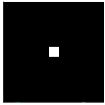
\includegraphics[width=0.5\linewidth]{env_examples/env0.png}
    \caption{Example of the simplest environment with a static square}
    \label{fig:env0}
\end{figure}

\begin{figure}
    \makebox[\textwidth][c]{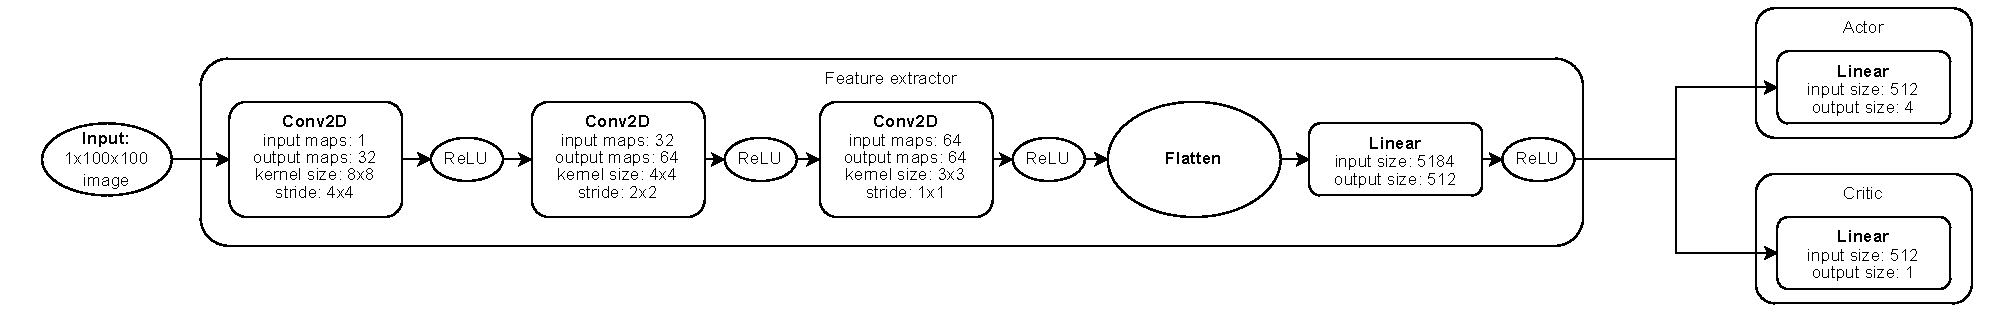
\includegraphics[width=1.5\linewidth]{diagrams/cnn_policy.pdf}}
    \caption{Architecture used by CNN policy. TODO make more readable somehow}
    \label{fig:cnn_policy}
\end{figure}

I expected the model to overfit very quickly since the state was always identical, and thus, there was one identical action that always yielded the best possible reward, but surprisingly, this did not happen, and the agent actually did pretty poorly, only managing to get an average IoU of 0.8. It also started to critically forget quite quickly, and it never recovered.

Figure \ref{fig:v0_rew} shows the mean reward per episode during the training. Since an episode always consists of exactly one observation, the biggest possible reward is 1 (since that is the highest score of IoU). The x-axis shows the elapsed timesteps. It reached its peak after around 180k episodes, and it never recovered.

\begin{figure}
    \centering
    \makebox[\textwidth][c]{\includesvg[width=1.25\linewidth]{graphs/v0_rew.svg}}
    \caption{The mean reward per episode for the simple static square environment}
    \label{fig:v0_rew}
\end{figure}


\subsection{Moving square of uniform size}
The next step forward was to make the square move. The initial state was created by randomly choosing a position within the image and placing the square there. All the other options (reward, action, and algorithm) remain the same. Some examples of this environment can be seen in figure \ref{fig:env1}.

\begin{figure}
    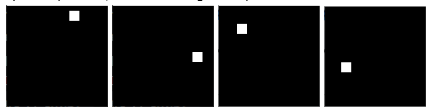
\includegraphics[width=1\linewidth]{env_examples/env1.png}
    \caption{Four examples of the environment with a moving square}
    \label{fig:env1}
\end{figure}

The best model was able to guess the position of the bounding box pretty well, usually within the actual square, but it struggled with the size even though, again, I expected it to overfit since there was a single correct answer. It even sometimes predicted the width or height of zero, even though that always resulted in a negative reward. Just like the previous model, this one also started catastrophically forgetting. In figure \ref{fig:v1_rew}, you can see the comparison between training in the two environments.

\begin{figure}
    \centering
    \makebox[\textwidth][c]{\includesvg[width=1.25\linewidth]{graphs/v1_vs_v0_rew.svg}}
    \caption{The mean reward per episode for the environment with moving square (orange) compared to the static square (gray)}
    \label{fig:v1_rew}
\end{figure}

\subsection{Moving rectangle}
\label{subsection:moving_rectangle}
The next environment was, once again, very similar, the only exception being that the object could now have any size, not just a perfect square of uniform size. \ref{fig:env2}

\begin{figure}
    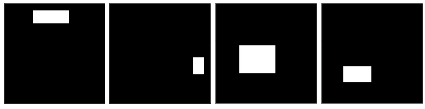
\includegraphics[width=1\linewidth]{env_examples/env2.png}
    \caption{Four examples of the environment with moving rectangles}
    \label{fig:env2}
\end{figure}

This time, I also wanted to try the other network architecture provided by the SB-3 library \texttt{MlpPolicy}, which has a simpler, non-CNN-based architecture shown in figure \ref{fig:mlp_policy}. It is simpler (1.3 million parameters compared to 2.7 million), but for such a simple problem, that could still be more than enough.

\begin{figure}
    \makebox[\textwidth][c]{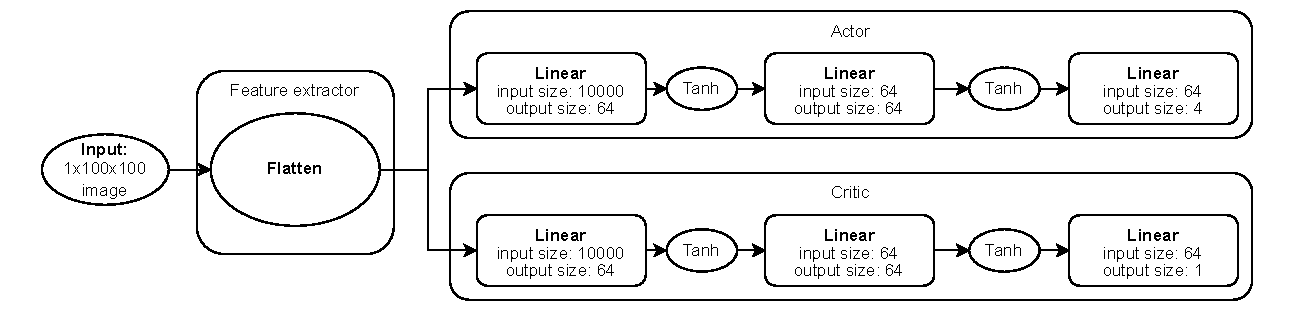
\includegraphics[width=1.5\linewidth]{diagrams/mlp_policy.pdf}}
    \caption{Architecture used by MLP policy.}
    \label{fig:mlp_policy}
\end{figure}

The MLP policy actually outperformed the CNN by a bit, and it also seemed a lot more stable. While it had some dips in its performance (probably caused by exploration), it always recovered and did not critically forget, as visible from figure \ref{fig:v2_mlp_cnn}.

\begin{figure}
    \centering
    \makebox[\textwidth][c]{\includesvg[width=1.25\linewidth]{graphs/v2_mlp_cnn.svg}}
    \caption{Comparison of the mean reward of the MLP policy (blue) and CNN policy (orange).}
    \label{fig:v2_mlp_cnn}
\end{figure}

\subsection{Multiple rectangles}
\label{subsec:multi-rect}
Since the performance of detecting a single object seemed pretty good, I decided to move on to more objects.
\begin{itemize}
    \item State: consists of a black 100x100 px image. Then, there are five attempts at placing a rectangle of random size in a random place. If it does not overlap with any already placed rectangle, it is added to the image. Because of this randomness, the amount of objects changes between episodes; it can be anywhere between 1 and 5, but on average, it is 3.5 objects. \ref{fig:env3}
    \item Action: the model returns 4 numbers representing the bounding box (x and y coordinates of the center and the width and height). If the predicted bounding box overlaps with any of the objects, that object is removed from the state (all of it, even if the prediction does not cover all of it)
    \item Reward: The reward calculation is very similar to the previous environments with just one object. If the prediction overlaps any objects, their IoU is the reward (if it overlaps multiple, then the maximum IoU is given). The episode is terminated when all objects are removed or stopped after $n$ guesses, where $n$ is the starting amount of objects. Note that the model is not directly punished for selecting more than one object, but since only one reward is given, it is more beneficial to select them separately since we want to maximize the cumulative reward during an episode.
\end{itemize}

\begin{figure}
    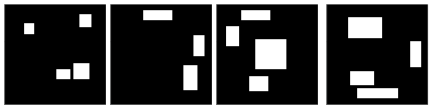
\includegraphics[width=1\linewidth]{env_examples/env3.png}
    \caption{Four examples of the environment with multiple moving rectangles}
    \label{fig:env3}
\end{figure}

Again, I tried both MLP and CNN strategies. The results can be seen in figure \ref{fig:v3_mlp_cnn}. At first glance, the results might seem just as good as in the previous environment, but remember that since the episodes last multiple timesteps (3.5 on average), the results are pretty poor as the maximum possible reward per episode is now around 3.5, whereas before, it was just 1. When we look at the episode length during training in figure \ref{fig:v3_len}, we can see that the model did use multiple steps for each episode, yet it still did not manage to achieve good results.

\begin{figure}
    \centering
    \makebox[\textwidth][c]{\includesvg[width=1.25\linewidth]{graphs/v3_mlp_cnn.svg}}
    \caption{Comparison of the mean reward of the MLP policy (blue) and CNN policy (red).}
    \label{fig:v3_mlp_cnn}
\end{figure}

\begin{figure}
    \centering
    \makebox[\textwidth][c]{\includesvg[width=1.25\linewidth]{graphs/v3_len.svg}}
    \caption{Comparison of the mean reward of the MLP policy (blue) and CNN policy (red).}
    \label{fig:v3_len}
\end{figure}

The next thing I tried was changing the definition of the action. Before, the four numbers represented the coordinates of the center along with the bounding box width and height. My thought process was that maybe the convolutional layers are not good at quantifying size; instead, they are better at finding a position of some pattern. So instead of center, height and width I changed the action to represent the coordinates of the top-left corner and the coordinates of the bottom-right corner. 

As can be seen in figure \ref{fig:v3_corner}, this change did help the CNN architecture model a bit but not by a lot. Surprisingly it made the MLP-based agent much worse.

\begin{figure}
    \centering
    \makebox[\textwidth][c]{\includesvg[width=1.25\linewidth]{graphs/v3_corner.svg}}
    \caption{Comparison of the mean reward of the MLP policy (cyan) and CNN policy (pink) when corners are used as the action.}
    \label{fig:v3_corner}
\end{figure}

Another idea I had was to utilize transfer learning. I did have a trained agent from the previous environment who was pretty good at finding one rectangle, so maybe if I used it here, it could use its already-learned knowledge and do better than the agents that started from the very beginning. The agent did start off much better than the new ones, but it quickly forgot everything and did not catch up. Below is the comparison of the transfer learning agent (blue) to the CNN-based agent shown before:

\begin{figure}
    \centering
    \makebox[\textwidth][c]{\includesvg[width=1.25\linewidth]{graphs/v3_transfer.svg}}
    \caption{Comparison of the mean reward of the original agent (pink) and the transferred agent (blue).}
    \label{fig:v3_transfer}
\end{figure}

In all of the charts, we can see that all the agents got to some point of knowledge relatively quickly, but after around 200k epochs, the progress slowed down massively or stopped completely. This could be due to the network being too simple to learn the problem, so I tried increasing the network size. Thankfully, this is relatively easy as SB-3 is based on PyTorch, so any kind of network can be passed to the training algorithm. As could be seen in figure \ref{fig:cnn_policy}, which shows the architecture of the CNN policy, both the actor and critic share a feature extractor, and then each of them only has one fully connected layer and nothing else, so it would be no wonder if they could not learn much.

In the new architecture, I added an extra layer to the shared feature extractor (poznámka: tohle byl spíš omyl, protože jsem moc nechápal co dělám xd) as well as adding two extra layers to each the actor and the critic. This meant that the model had around 6 million parameters. The model now had the architecture shown in figure \ref{fig:bigger_net_policy}.

\begin{figure}
    \makebox[\textwidth][c]{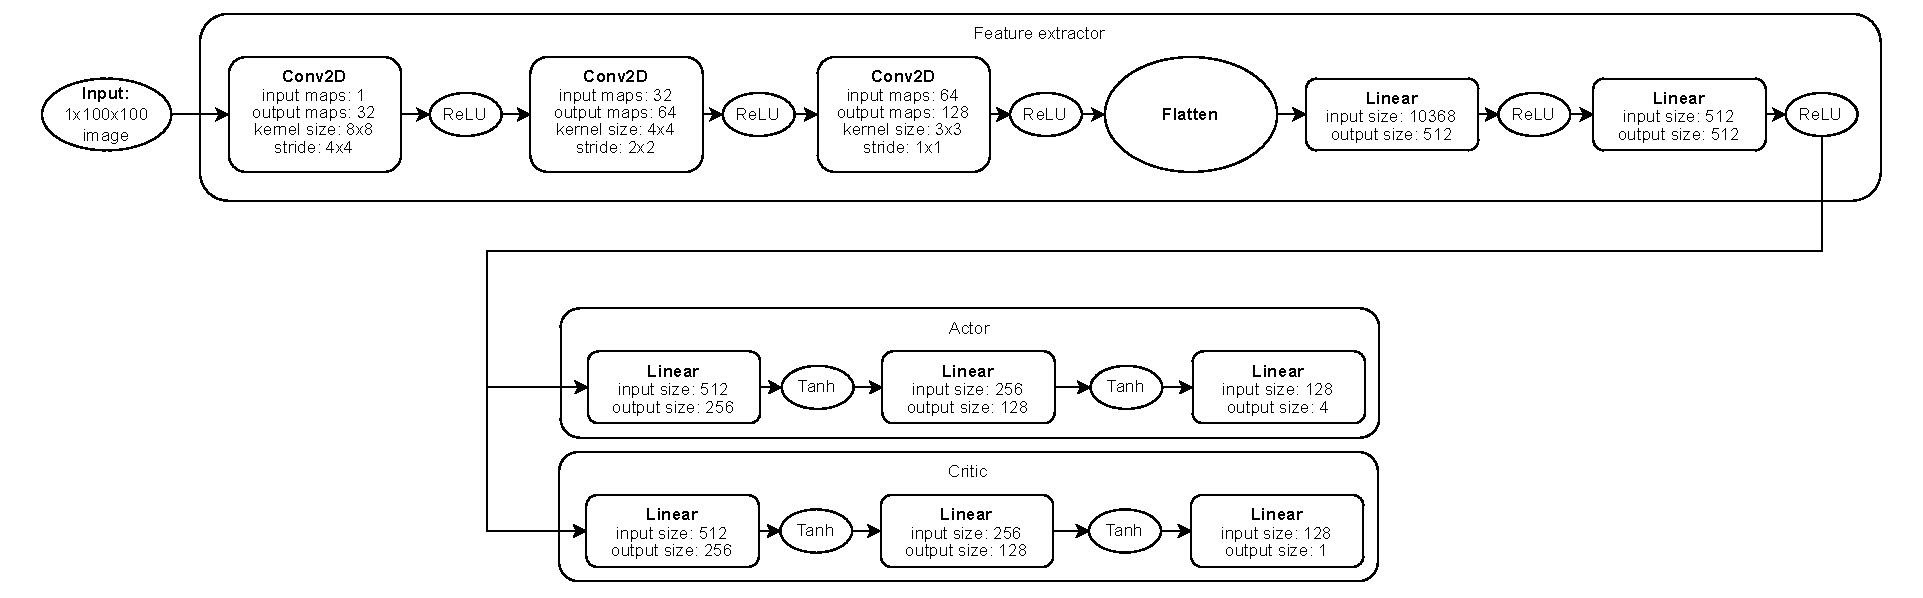
\includegraphics[width=1.5\linewidth]{diagrams/bigger_net_policy.pdf}}
    \caption{New CNN-based policy with larger networks for actor and critic.}
    \label{fig:bigger_net_policy}
\end{figure}

This change helped quite a bit. It performed the same as the simple networks in less than 6 times the number of episodes, and it continued learning even after more than 7 million episodes. Figure \ref{fig:v3_bigger_net} shows the comparison between the bigger network, the best MLP policy model, and the best CNN policy model. The mean episode lengths did not differ dramatically.

\begin{figure}
    \centering
    \makebox[\textwidth][c]{\includesvg[width=1.25\linewidth]{graphs/v3_bigger_net.svg}}
    \caption{Comparison of the bigger network (orange), best small MLP model (blue), and best small CNN model (pink).}
    \label{fig:v3_bigger_net}
\end{figure}

The resulting model took around 6 hours to train and reached a mean reward of around 2.1 per episode or an average IoU of 0.6. While this might still sound pretty bad, note that because of the small size of the image, IoU is pretty strict. For example, if for a rectangle of size 20x20, we guessed a bounding box of the correct size but shifted to the left and down by 2 pixels, the IoU would be only 0.68 even though the guess is only off by 10  \%. Another problem that brings the average down is that sometimes when the image contains two objects far apart, the model gets confused and predicts a bounding box between them repeatedly until the episode is stopped; an example of this behavior can be seen in figure \ref{fig:v3_stuck}.

\begin{figure}
    \centering
    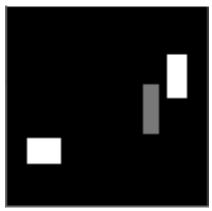
\includegraphics[width=0.5\linewidth]{results/v3_stuck.png}
    \caption{Example of the model getting stuck when two objects are far apart. White rectangles are the actual objects, and grey is the prediction.}
    \label{fig:v3_stuck}
\end{figure}

\subsection{Different shapes}
Now that the model was able to predict multiple rectangles in a single image with quite good success, the next step was to introduce other shapes as well. The environment is identical to the previous one, but now, instead of just rectangles, there could also be ellipses and triangles (both of any size and four different possible orientations). Since the rules were still the same, there were an average of 3.5 objects, and they did not collide. Some examples of this environment can be seen in figure \ref{fig:env4}.

\begin{figure}
    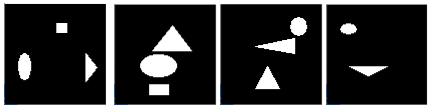
\includegraphics[width=1\linewidth]{env_examples/env4.png}
    \caption{Four examples of the environment with a moving square}
    \label{fig:env4}
\end{figure}
 
The training on my bigger network started off very similarly to the previous environment, but it never reached quite the same results as can be seen in figure \ref{fig:v4_bigger_net}.

\begin{figure}
    \centering
    \makebox[\textwidth][c]{\includesvg[width=1.25\linewidth]{graphs/v4_bigger_net.svg}}
    \caption{Comparison of the environment with just rectangles (orange) and with other shapes (pink).}
    \label{fig:v4_bigger_net}
\end{figure}

Since the problem is similar to the previous one, I again tried to use transfer learning with the best model from the previous environment for the new one. It actually started with very good results and stayed there for the rest of the training, only improving a little bit, see figure \ref{fig:v4_transfer}.

\begin{figure}
    \centering
    \makebox[\textwidth][c]{\includesvg[width=1.25\linewidth]{graphs/v4_transfer.svg}}
    \caption{Comparison of the rectangle-only environment (brown), model with other shapes from scratch (pink) and transferred (blue).}
    \label{fig:v4_transfer}
\end{figure}

This showed me that it was definitely possible to get good results. But I wanted to avoid transfer learning, if possible, until the very end because if it were needed this early on, it would create a very long and impractical chain of models that depend on one another. For those reasons, I wanted to improve the network further. It is a common practice not to create your own feature extractor but instead to use an already existing convolutional network trained by someone else, remove the last layer, and use that as a feature extractor [Source???]. I wanted to try exactly that.

ResNet18 is a model architecture first proposed in the paper Deep Residual Learning for Image Recognition (\url{https://arxiv.org/abs/1512.03385}). The architecture of ResNet18 is shown in figure \ref{fig:resnet}, source (\url{https://www.researchgate.net/figure/Proposed-Modified-ResNet-18-architecture-for-Bangla-HCR-In-the-diagram-conv-stands-for_fig1_323063171}).

\begin{figure}
    \centering
    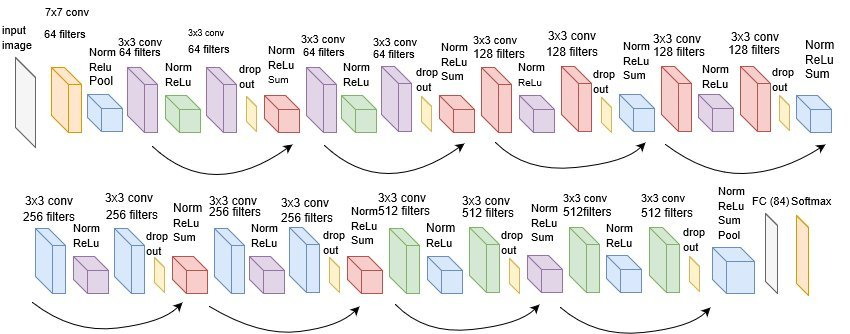
\includegraphics[width=1\linewidth]{diagrams/resnet.png}
    \caption{Architecture of ResNet18}
    \label{fig:resnet}
\end{figure}

Most notably, it contains 18 convolutional layers (hence the 18 in the name), batch normalization after most of the convolutional layers, and skip connections which allow some of the input to skip the layers, which helps with vanishing gradient. Also, at the end, we can see an adaptive average pooling layer. Unlike regular pooling layers, this one has the output size as a parameter and chooses the stride and kernel size automatically based on the input. This means that we can pass any size of input into it, and the output will be the same size. To use it in our model, we cut off its last fully connected layer.

A slight complication is that ResNet18 is meant for colored images (3 channels), but we are currently using binary grayscale images (1 channel), although this might change in the future. There are multiple ways of solving this problem; the simplest is to just duplicate the one channel 3 times. I did something a bit different, adding a convolutional layer at the beginning with a kernel of size 1x1x3, which creates 3 feature maps from our one image. This is very similar to just duplicating the channel 3 times, but the kernel contains learnable parameters, so it is possible for the channels to be different if the network finds that useful. The entire architecture is shown in figure \ref{fig:resnet_policy}.

It is also important to note that the pre-trained ResNet18 (provided by PyTorch) was trained on the COCO dataset, which consists of photographs. This could mean it does not perform as well on binary images (and later on images of websites), but for now, that hopefully should not be a problem.

\begin{figure}
    \centering
    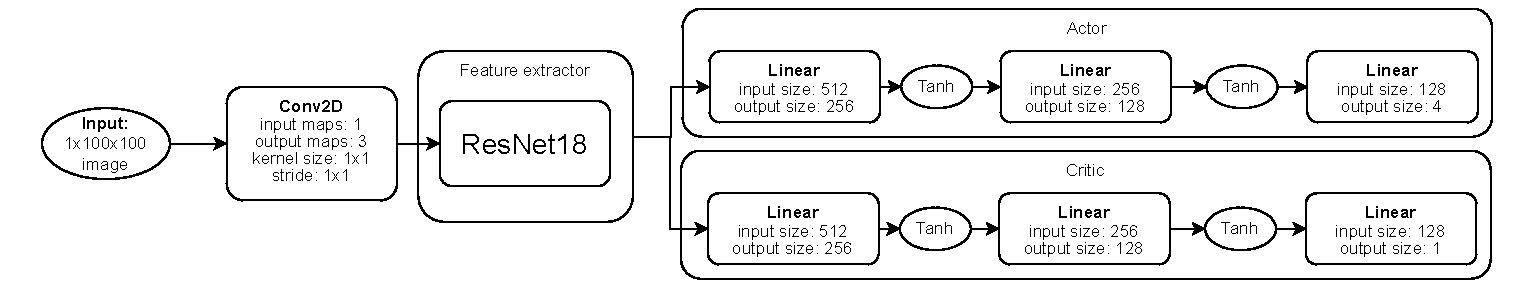
\includegraphics[width=1\linewidth]{diagrams/resnet_policy.pdf}
    \caption{The new architecture, using ResNet18 as a feature extractor. TODO make more readable}
    \label{fig:resnet_policy}
\end{figure}

A notable effect of this change is that the training is now around 3 times slower (which means 1 million timesteps now take around 2.5 hours on my computer. Hopefully, this could be offset by the improved performance).

I tried again on the same environment, and the results were not great, as visible in figure \ref{fig:v4_resnet_frozen}. I was very surprised by how poor the results were, but I soon found the cause. As the ResNet18 feature extractor was already pre-trained, I thought freezing its weights would make the training faster while not really affecting the results, but I was very wrong. When I tried training again, this time with the weights unfrozen, I got a much better result shown in figure \ref{fig:v4_resnet_finetune}.

\begin{figure}
    \centering
    \makebox[\textwidth][c]{\includesvg[width=1.25\linewidth]{graphs/v4_resnet_frozen.svg}}
    \caption{Comparison of the old network trained from scratch (pink), transferred model (blue) and new network with ResNet18 feature extractor (cyan).}
    \label{fig:v4_resnet_frozen}
\end{figure}

\begin{figure}
    \centering
    \makebox[\textwidth][c]{\includesvg[width=1.25\linewidth]{graphs/v4_resnet_finetune.svg}}
    \caption{Comparison of the old network trained from scratch (pink), transferred model (blue) and new network with ResNet18 feature extractor (grey).}
    \label{fig:v4_resnet_finetune}
\end{figure}

It got the same result as the current best model in just above 500k timesteps, and it even overtook it by a noticeable margin. Sure, the new network was slower to train, but since the previous best model was transferred, it also needed its previous model, so in total, the training was actually faster.

I also wanted to check whether this improvement was caused by the feature extractor being pre-trained or just by the network being significantly bigger. So I repeated the same exact training, but this time with ResNet18 not being pre-trained. In figure \ref{fig:v4_resnet_from_scratch} is the comparison of my old architecture being trained from scratch compared to the new architecture being trained from scratch. We can see that the results are very similar, so I can confidently say that a pre-trained feature extractor does indeed make a difference, although it still has to be fine-tuned.

\begin{figure}
    \centering
    \makebox[\textwidth][c]{\includesvg[width=1.25\linewidth]{graphs/v4_resnet_from_scratch.svg}}
    \caption{Comparison of the old network trained from scratch (pink) and the new network with the ResNet18 feature extractor being trained from scratch (orange).}
    \label{fig:v4_resnet_from_scratch}
\end{figure}

\subsection{Hollow shapes}
Since it is important for the final model to be able to detect objects located inside one another (to deduce their hierarchy), the next step I wanted to try was to do exactly that -- include shapes inside other shapes. But to do that, I would first need the objects to be hollow. Some examples can be seen in figure \ref{fig:env5}.

\begin{figure}
    \centering
    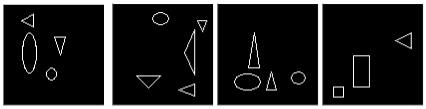
\includegraphics[width=1\linewidth]{env_examples/env5.png}
    \caption{Four examples of the new environment}
    \label{fig:env5}
\end{figure}
 
I believed that this change would have little to no impact, but I still wanted to try, just in case. However, as expected, this had almost no impact on the training (gray is the old environment, and blue is the new one with hollow shapes), although we can see a couple more dips in figure \ref{fig:v5}.

\begin{figure}
    \centering
    \makebox[\textwidth][c]{\includesvg[width=1.25\linewidth]{graphs/v5.svg}}
    \caption{Comparison of the old environment with filled-in shapes (gray) and the new with hollow shapes (blue)}
    \label{fig:v5}
\end{figure}

\subsection{Bigger images}
One thing that is still very different between my prototype and what should be the final product is the size of the input image. AIVA currently mostly uses images in the FullHD format (1920x1080px). Of course, some downscaling is possible if we do not need great details (for example, for reading small text), but downscaling the image all the way to 100x100px would most likely not work very well, and the aspect ratio is also wrong. For these reasons, I wanted to try making the input image larger and see if the current model can work with them just as well as with the smaller ones. Thanks to the aforementioned adaptive pooling layer in ResNet18, I only needed to change the size of the observation space.

At first, I wanted to go all the way to FullHD or at least to HD, but unfortunately, this was not possible due to hardware limitations. The training used all of the GPU's dedicated RAM (10 GB) as well as the shared RAM (16 GB) and then crashed. The largest resolution I managed to get working was 480p (640x480px), and even then, I had to cut the batch size in half (from 64 to 32). Since the image was bigger I also increased the amount of objects on it on average from 3.5 to 15.

The training started similarly to the previous ones, but it got stuck pretty quickly and did not improve much afterward. I stopped the training after just around 300k episodes. It is possible that the model would catch up eventually, but this setup was not good for experiments since it was over ten times slower than before. For those reasons, I reduced the image size to 200 by 200 pixels, which only slowed down the training by about two times. But even then, the results were not great. From testing the model, it seems that they learned that placing large bounding boxes in places where something is located gives positive rewards, and they did not explore enough to realize that selecting each individually gives a much bigger reward. 

Remember that the current reward function did not punish selecting multiple bounding boxes in any way. So I decided to try and modify it. This would, hopefully, incentivize the model to really avoid selecting multiple objects at once. I came up with the following two possible modifications:
\begin{itemize}
    \item The item with the biggest overlap minus the overlaps of all the other items divided by the union of the main object and the guess
    \item Calculate IoUs of all intersecting objects. The reward is the biggest IoU minus the sum of all the other IoUs multiplied by some constant.
\end{itemize}

I then let it train using all three of the reward functions for around 2.5m episodes. Of course, RL training can be somewhat unstable, so it would be better to run this experiment multiple times, but it should show us if there are any major differences between the reward functions.

I then benchmarked the three models (this time with the same reward function, otherwise it would not be fair) by running 5000 episodes. The best performing was the method punishing overlap, which scored on average 4.6 per episode (0.59 per object). The other two methods scored similarly -- the one that did not punish scored on average 3.9 per episode (0.5 per object), and the one that punished much harsher scored an average of 4.0 per episode (0.51 per object). There was very little difference in the average episode length.

\subsection{Hierarchical environment}

So far all the environments comprised of objects that did not intersect in any way. They were completely independent, and thus, the order in which they were selected did not matter at all. This, of course, differs from how real websites look. They have a hierarchy of objects (one object can contain many others). The next step was to create an environment that would represent this more faithfully.

At first, I tried to use the same technique as before -- randomly attempting to place objects that do not overlap, but this time, I allowed such overlaps where one object was fully inside another. This did not work very well; the number of objects differed greatly between attempts, they were often placed very close to one another, and the depth of the hierarchy was very shallow. So instead, I created a generator that directly created a tree-like structure. It starts with a root object that encloses the whole image, then it selects an area inside with a random offset to the parent object and randomly selects the number of children, their sizes, and the spacing between them. The algorithm then does this recursively for each child. It is also possible to customize the maximum depth, the minimum size of an object, minimum spacing, and so on. Some examples of this new generation can be seen in figure \ref{fig:env7}

\begin{figure}
    \centering
    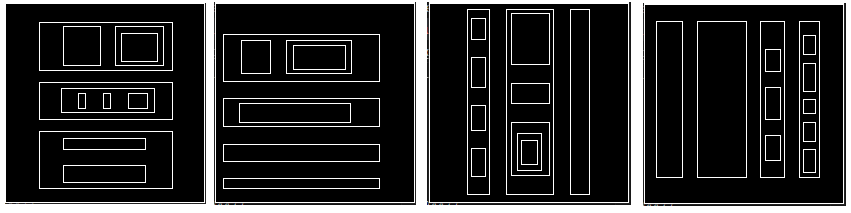
\includegraphics[width=1\linewidth]{env_examples/env7.png}
    \caption{Four examples of the new environment}
    \label{fig:env7}
\end{figure}

A new reward function was needed as well. I came up with the following method. First, find all objects that the guess intersects with or fully encloses; if there are none, also include objects that fully enclose the guess (there will always be at least the root). If there is just one such object, the reward is the IoU of the guess, and this object minus the percentage of its area occupied by its children that have not been guessed yet (this is to discourage selecting objects that still have children). This object is then removed (including all of its children). If there are multiple intersecting objects, then the one that is deepest in the hierarchy is chosen, and the same calculations are done. The episode ends when the root object is removed.

I tested this new environment by training two new models. One from scratch and the other transferred from the previous environment. After around 7 million time steps, they both managed to get an average reward of about two. The transferred model did do better by around 25 percent but both did pretty bad. From the testing, it was clear that the model learned that placing long bounding boxes of width zero would almost always result in a nonnegative reward because the IoU of such bounding box is always zero, and the model did not explore enough to realize that it could do much better.

To combat this, I tried modifying some hyperparameters that should encourage exploration, namely:
\begin{itemize}
    \item The discount factor $\gamma$ (described in section \ref{section:goal}) -- by default, this parameter is set to 0.99, but in our case, discounting does not really make sense. Because of how the environment is set up, the maximum number of steps for the episode is capped, and an ideal policy will use up all of them. Thus, discounting is not needed, and $\gamma$ should be set to 1.
    \item Entropy loss coefficient $c_2$ -- in the PPO loss function contains an entropy bonus which rewards less deterministic policies. Increasing it should thus lead to more exploration \cite{PPO_paper}
    \item Clipping range $\epsilon$ -- One of the main benefits of PPO is its clipping function that prevents big updates to a policy, which should prevent it from \enquote{jumping off a cliff} \cite{PPO_paper}. By increasing it, the training might become more unstable, but it also might help to get out of local maxima.
    \item Learning rate $\varepsilon$ -- When making an update to the policy network, the gradient is multiplied by this constant. Higher learning should make the training faster, but at the same time, the jumps are bigger, which can lead to unstable learning.
\end{itemize}

I tried both lowering and increasing each of these parameters but unfortunately, none of the changes had a bigger positive impact. Lowering $\gamma$ and increasing the clip range did lead to slightly better results but only by a little. This showed me that it might be better to try a completely different approach rather than trying to improve this one over and over with little to no success.

\chapter{Training a model that predicts iteratively}
\label{chap:iterative}

Since the results of the previous approach, which guessed bounding boxes directly (one action = one prediction), did not work well, especially in a more complex environment, I wanted to try a different approach. \cite{rl_object_detection} describes and compares two approaches for object detection using reinforcement learning, both using discrete action space (which should be a bit simpler for the model to learn). Both of these methods start with a bounding box spanning the entire image, and the agent chooses actions to modify this box repeatedly until it is happy with the prediction, at which point it selects the \texttt{trigger} action, which ends the episode and grants the final reward.

The first method, originally described in \cite{hierarchical_od_with_drl}, has five movement actions (each results in zooming into a different 'quarter' of the image) and a stop action. It showed promising results on a single object, single class object detection, but it is unusable for our purpose since it only produces bounding boxes with one fixed aspect ratio.

The second method, originally described in \cite{iterative_od_with_rl}, uses a similar approach but instead of five actions for zooming in different areas, it has a total of eight movement actions (plus the trigger), four of which move the bounding box (up, down, left and right), two for size changes (zoom in, zoom out) and two for aspect-ratio changes (making the box fatter or taller). This allows for way more flexibility, although some bounding boxes are still impossible because the changes are of some fixed size, but if this size is small enough, we should be fine as we probably do not need pixel-perfect predictions. An example of one episode can be seen in figure \ref{fig:exmaple_from_paper}.

\begin{figure}
    \centering
    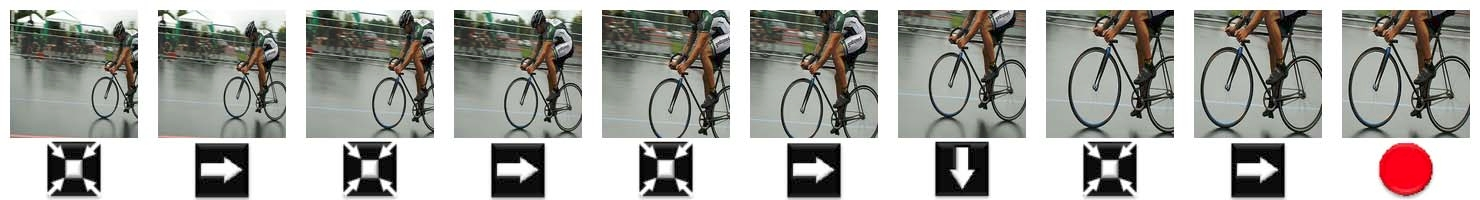
\includegraphics[width=1\linewidth]{diagrams/45.jpg}
    \caption{Example of taken actions to locate and object \cite{iterative_od_with_rl}}
    \label{fig:exmaple_from_paper}
\end{figure}

As for the observation space, it is once again an image, but this time only the part that is inside the current bounding box scaled up to some fixed size since regular RL algorithms do not allow for an input of variable size. The original paper \cite{iterative_od_with_rl} also used a vector of ten previous one-hot encoded actions but \cite{rl_object_detection} found that including them did not help.

I implemented this approach in a simplified form as a proof of concept with only four actions, each of them shrinking the bounding box by some fixed percentage from one of the four sides and the trigger action. This simplifies the problem while keeping the ability to create predictions of any size.

The suggested reward function compares the IoU of the state before and after an action is taken and gives a reward of +1 if the action improved the guess and -1 if it got worse. When the trigger action is taken, a reward of $\eta$ is given if the resulting IoU is over some threshold $\tau$, $-\eta$ otherwise. The suggested values are $\eta=3$, $\tau=0.5$. \cite{rl_object_detection} further tried changing them but did not find any improvements when they were increased.

This reward function is good for single object detection because the correct action will always improve the IoU, but when multiple objects are present, and the calculation is more complicated than IoU, this does not have to be the case. For this reason, I started my PoC with a much simpler sparse reward function, which only gives a reward for the trigger action using the same calculation as in my previous environments.

The first experiment I did was on one of the simplest environments I made, containing just one filled-in rectangle of variable size at variable position (described in \ref{subsection:moving_rectangle}). The model learned to find the rectangle pretty quickly, but the accuracy was not great, mainly because the bounding box modification step was too large (one step shrunk the bounding box by 15 \%). When I lowered it to just 5 \%, the accuracy improved, but it took way too many steps (around 60), which would later slow down the inference by a lot. For this reason, in the following environments, I implemented two actions per direction, one shrinking the bounding box by 15 \% and one by just 2.5 \%. This does make the task slightly more complex but, at the same time, allows for precise predictions with a low amount of steps.

I then moved on to the next environment described in \ref{subsec:multi-rect}, which contains multiple rectangles. With the default hyperparameters, it struggled, but when I tried running it with a higher clip range and lower gamma (as discovered in the previous chapter), all of a sudden, the results were much better. There was no big change when I changed the rectangles to be just outlines.

With the hierarchical environment, it once again struggled, so since I saw how big of an impact hyperparameters can have, I decided to once again try to tune them. But this time not using just manual guessing but instead an automated process. The SB-3 documentation recommended to use the rl-zoo library, which contains pre-trained models, environments, and scripts for training and hyperparameter optimization. I tried using it but failed to use it for my more complicated network architecture. So instead I wrote my own script.

\section{Optuna}
Optuna\footnote{\url{https://optuna.org/}} is an open source framework for automated hyperparameter search. It uses state of the art algorithms to suggest hypermarameters based on previous experiences making it much more time efficient than usual methods such as grid-search. 

Using it is very simple. You just need to define an \texttt{objective} function that takes a \texttt{trial} object as input, uses this trial object with methods like \texttt{trial.suggest\_int} or \texttt{trial.suggest\_categorical} to get the suggested hyperparameters and returns a float representing how well the objective was met (this is most often some accuracy metric, in our case it is the mean per episode reward). A study is then created using the \texttt{optuna.create\_study} function. This study can then be optimized for some amount of trails after which it returns the best found hyperparameters.

A study can also be connected to a relational database where it logs all the trails. This can be then fed to Optuna dashboard\footnote{\url{https://optuna-dashboard.readthedocs.io/en/latest/getting-started.html}} which can visualize information such as hyperparameter importance, plots of the tuning progression and much more.

It is also possible to run multiple Optuna instances in parallel, all using the same database, which allows for very simple way of distributed tuning on multiple machines with almost linear scaling.

Another great feature is the possibility of pruning. In cases where the objective function has some intermediate values (for example accuracy after each epoch), Optuna can stop the trail early when the results after some amount of training are not close to the current best which greatly reduces the overall tuning time.

I ran a study of around 100 trails each consisting of at most 200,000 episodes reporting intermediate values every 20,000 episodes. On two computers this took around 6 hours. The progress can be seen in figure \ref{fig:optuna-progress}. Optuna was allowed to tune almost every possible hyperparameter of the PPO algorithm including things like size of the actor and critic networks. From the results it was clear that learning rate made the biggest difference. Up until this point I only used fixed learning rate but Optuna found much better results using linear decaying learning rate.

\begin{figure}
    \centering
    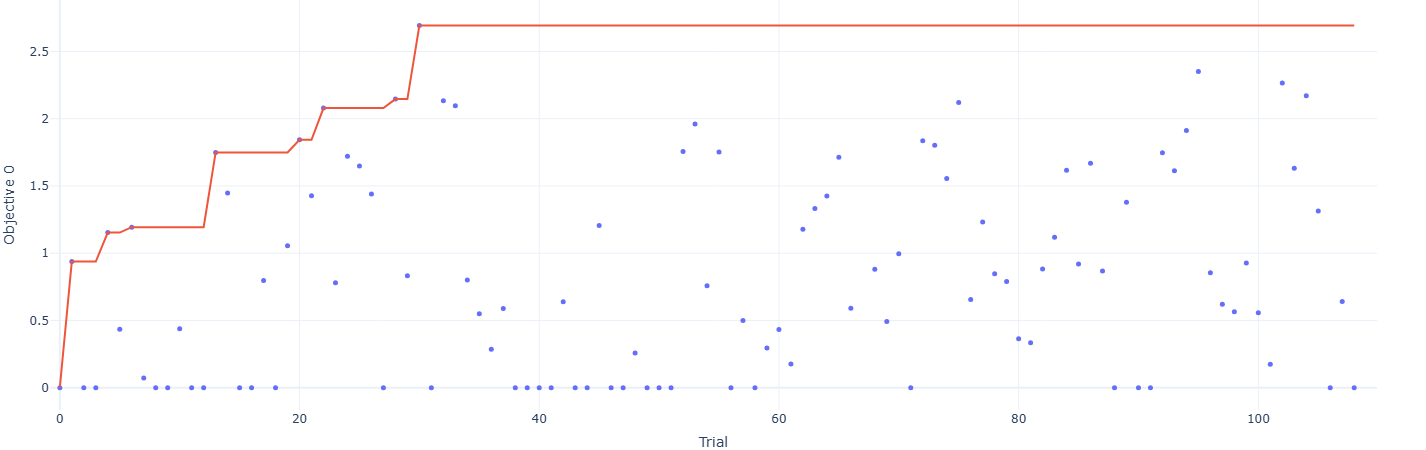
\includegraphics[width=1\linewidth]{diagrams/optuna_progress.png}
    \caption{Progress of hyperparameter tunning with Optuna}
    \label{fig:optuna-progress}
\end{figure}

\chapter{Comparison with other methods}
TODO: Implement two solutions: one based on CNNs (probably YOLOv8 with some free dataset), one based on classical CV (finding contours).
%
Compare how hard (and time consuming) it was to make compared to the RL solution and how the result compares (do not forget to mention biases and differences).


\printbibliography[heading=bibintoc] %% Print the bibliography.


\appendix %% Start the appendices.
\chapter{An appendix}
Here you can insert the appendices of your thesis.

\end{document}
